\section{Operaciones matemáticas}

Además de las operaciones vectoriales básicas que ya vimos, existen las funciones universales, mejor conocidas como \textit{ufuncs}. Lo más importante que debe saber es que estas funciones se aplican de manera vectorizada.

Si usted quisiera sacar la raíz cuadrada de 100 datos a mano, tendría que sacar la calculadora y empezar a pelearse con cada número. Pero como usted no quiere entregar su análisis un semestre más tarde, utiliza \textit{NumPy}, que aplica la operación a todo el vector, matriz o tensor elemento por elemento sin perder ni un ápice de eficiencia. ¡Si no fuera así, usaríamos la librería \textit{math} y nos iríamos a dormir una siesta mientras la computadora procesa!.

\subsection{Raiz cuadrada y exponencial}

Estas son las funciones "base" para una infinidad de cálculos estadísticos, financieros y científicos.
\begin{itemize}
    \item Raiz cuadrada: \textit{np.sqrt}, que calcúla \(\sqrt{x}\) para cada elemento.
    \item Exponencial: \textit{np.exp}: calcula \(e^x\) (donde \(e\) es el numero de Euler). Esta función es fundamental para calcular intereses compuestos, crecimientos poblacionales o para cuando su código decide crecer exponencialmente en errores. Podría dedicar toda una sección a explicar la belleza de\(e^x\), pero lamentablemente este no es un libro de álgebra y ambos tenemos cosas mejores que hacer.
\end{itemize}

Veamos estas operaciones en acción en su hábitat natural:
\begin{pycode}{Raiz y Exponencial}

import numpy as np

arr = np.array([1, 4, 9, 16])

# Raíz cuadrada
raices = np.sqrt(arr) # [1., 2., 3., 4.]

# Exponencial (e^x)
exp_valores = np.exp(np.array([0, 1, 2])) # [1., 2.718..., 7.389...]

\end{pycode}

Observe que los resultados son siempre \textit{floats} (decimales). NumPy sabe que las raíces y las exponenciales rara vez son exactas, así que se prepara para la imprecisión de la vida real desde el principio.



\subsection{Logaritmo Natural}

Si en matemáticas \(e^x\) nos dice cuánto creció una población en un tiempo determinado, el logaritmo natural \((ln(x))\) nos dice cuánto tiempo tuvo que pasar para alcanzar ese crecimiento.

Básicamente, el logaritmo natural es como un domador de monstruos numéricos. Se usa principalmente para:
\begin{itemize}
\item \textit{Normalizar escalas:} Si tiene datos que van de 1 a 1,000,000 (como seguidores en TikTok o la deuda externa), graficarlos es un caos visual. El logaritmo "aplasta" los números gigantes y "estira" los pequeños, haciendo que todo quepa elegantemente en una gráfica.
\item \textit{Linealizar relaciones:} Convierte curvas exponenciales complejas en líneas rectas, lo cual es oro puro para entrenar algoritmos de Inteligencia Artificial sin que su computadora explote en el intento.
\item \textit{Interés compuesto:} Fundamental para calcular cuánto tiempo tardará en ser millonario si decide invertir sus ahorros en lugar de gastárselos en café.
\end{itemize}
    

Imagine que se generó una colonia de bacterias que crece de forma masiva \((e^x)\) y usted quiere saber qué tan rápido fue ese crecimiento. Utilizando \textit{np.log()}, podemos estimar esos tiempos de la siguiente manera:

\begin{pycode}{Logaritmo natural}
import numpy as np

# Cantidad de bacterias en diferentes muestras
bacterias = np.array([1, 10, 100, 1000])

# Aplicamos el logaritmo para "suavizar" los datos
tiempos_estimados = np.log(bacterias)

print(tiempos_estimados)
# Resultado: [0. , 2.30258509, 4.60517019, 6.90775528]
\end{pycode}

Observe cómo pasamos de una escala que saltaba de 10 en 10 (multiplicando) a una escala lineal que avanza de forma constante. Eso es \textit{NumPy} poniendo orden en el caos.

\begin{nota}
    \textbf{Advertencia:} El logaritmo natural es una función muy útil, pero tiene un temperamento difícil: no acepta números negativos ni el cero. Si intenta calcular \textit{np.log(0)}, \textit{NumPy} le devolverá un \(-\infty\) (\textit{infinito negativo}) y un aviso de que algo está muy mal en su vida (o al menos en sus datos).
\end{nota}


\subsection{Funciones trigonométricas}

Imagine que tiene un asador de pollos giratorio. Las funciones trigonométricas no son más que las coordenadas que nos dicen dónde está el pollo en cada momento mientras da vueltas en un círculo unitario.

Imagine un círculo cuyo radio es exactamente 1. El pollo empieza a la derecha y gira en sentido contrario a las agujas del reloj. El ángulo (\(\theta\)) es qué tanto ha girado el asador.

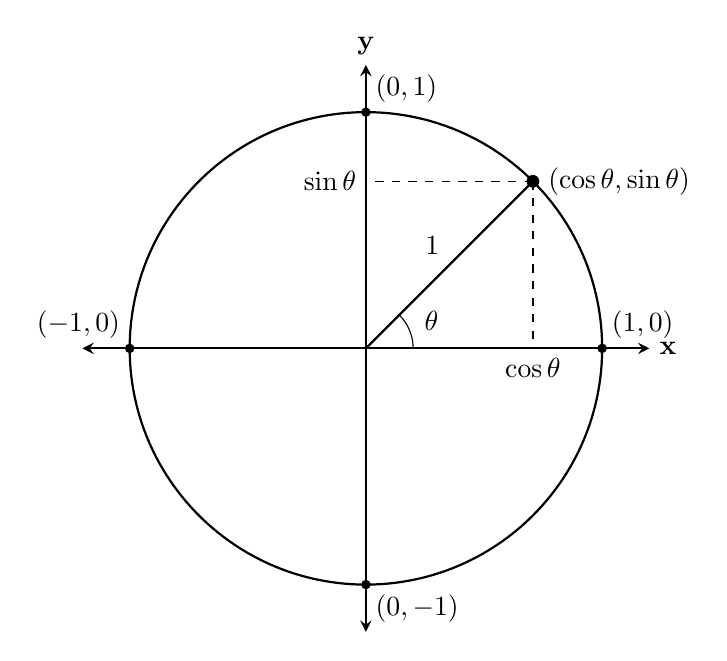
\begin{tikzpicture}[>=stealth, scale=3]

    % Dibujar los ejes X e Y
    \draw[<->, thick] (-1.2, 0) -- (1.2, 0) node[right] {\textbf{x}};
    \draw[<->, thick] (0, -1.2) -- (0, 1.2) node[above] {\textbf{y}};

    % Dibujar el círculo unitario
    \draw[thick] (0,0) circle (1);

    % Definir variables para el ángulo
    \def\angle{45} % Puedes cambiar este valor para mover el punto
    \def\radius{1}

    % Dibujar el radio (línea desde el origen al punto)
    \draw[thick] (0,0) -- (\angle:\radius) node[midway, above left] {1};

    % Dibujar las líneas discontinuas (proyecciones)
    \draw[dashed] (\angle:\radius) -- ({\radius*cos(\angle)}, 0) node[below] {$\cos \theta$};
    \draw[dashed] (\angle:\radius) -- (0, {\radius*sin(\angle)}) node[left] {$\sin \theta$};

    % Dibujar el arco del ángulo theta
    \draw (0.2,0) arc (0:\angle:0.2);
    \node at (22.5:0.3) {$\theta$};

    % Dibujar los puntos negros en las intersecciones de los ejes
    \filldraw (1,0) circle (0.5pt) node[above right] {$(1, 0)$};
    \filldraw (-1,0) circle (0.5pt) node[above left] {$(-1, 0)$};
    \filldraw (0,1) circle (0.5pt) node[above right] {$(0, 1)$};
    \filldraw (0,-1) circle (0.5pt) node[below right] {$(0, -1)$};
    
    % Dibujar el punto sobre el círculo y su etiqueta
    \filldraw (\angle:\radius) circle (0.7pt) node[right, xshift=2pt] {$(\cos \theta, \sin \theta)$};

\end{tikzpicture}

Hay tres funciones principales:
\begin{itemize}
    \item Seno \(\sin\): Es la altura del pollo. Cuando el ángulo es 0°, la altura es 0. Cuando llega arriba (90°), la altura es 1.
    \item Coseno \(\cos \): Es la distancia horizontal desde el centro. Cuando el ángulo es 0°, el pollo está todo a la derecha (1). A los 90°, está justo en el centro horizontal (0).
    \item Tangente \(\tan\): Es la relación entre la altura y la distancia. Imagina la sombra que proyecta el pollo en una pared vertical lejana.
\end{itemize}

Si usted no es ingeniero ni arquitecto, podría pensar que esto no tiene utilidad en el análisis de datos. Se equivoca: la trigonometría está en todas partes, desde el procesamiento de audio y música, hasta el análisis de ciclos eléctricos, señales de radio y física de videojuegos.

\begin{nota}
    En \textit{NumPy}, las funciones esperan que les hables en Radianes, no en grados. \(180°= \pi\) radianes (aprox. 3.14159).
\end{nota}

Veamos cómo interrogar al pollo en código:

\begin{pycode}{Funciones trigonométricas}
import numpy as np

# Queremos saber la altura del pollo a los 90 grados
angulo_grados = 90
angulo_rad = np.radians(angulo_grados) # Convertimos a radianes

altura = np.sin(angulo_rad)
distancia = np.cos(angulo_rad)

print(f"A los 90°, la altura (Seno) es: {altura}") # Debería ser 1.0
print(f"A los 90°, la distancia (Coseno) es: {distancia}") # Debería ser casi 0
\end{pycode}

Como habrá notado, el coseno de 90° no dio exactamente 0, sino un número absurdamente pequeño \((6.12\times10^{-17})\). Esto sucede porque las computadoras tienen limitaciones de precisión decimal. No se asuste; para nosotros, eso es cero.

Existen miles de funciones como \textit{np.radians} o \textit{np.degrees} que no vamos a abarcar aquí. Si pretendiera explicar cada función de la librería, este apunte tendría más hojas que la documentación oficial y usted se quedaría sin espacio en su disco duro. Cuando necesite algo muy específico, no dude en consultar la documentación de \textit{NumPy}.

